\chapter{Experiments \& Results}\label{chapter:experiments}

This chapter covers what experiments were run to test the performance of the different types of cox control policies. Schedules were created for these experiments with different numbers of boats and different delays between boat launch. Data were collect for simulation runs of each of theses schedules using different control policies. These data were then analysed from different perspectives to determine the relative strengths and weaknesses of each type of control policy.

\section{Overview of experiments run}
  For each experiment the simulation was run with a variety of
  differing starting parameters. Each experiment then examined a
  different aspect of the boat's behaviour. The sets of simulation
  parameters used for experiments are described next. Then there is a
  brief overview of the experiments carried out.

  \subsection{Simulation Parameters}
  For the experiments, the simulation was setup according to the
  parameters associated with a single row in the
  simulation\_parameters table. These parameters are the control
  policy, the random seed and the launch schedule to use. The launch
  schedule is made of up lists of parameters for each boat to be
  launched. These are the launch tick, desired gear, the speed
  multiplier and the minimum distance to cover for each boat in the
  schedule. These parameters are described in more detail in Section \ref{software:experiment:db}.
  
  The launch schedules were created by specifying a number of boats
  and a fixed delay between each boat launch. Each boat was assigned a
  desired gear between 1 and 10 uniformly at random. The speed
  multiplier was fixed at 0.5 (corresponding to a top speed of 5m/s,
  which matched the fastest time set by crew racing the course on
  April 28th 2012). The distance to cover was fixed at 5000m which is
  roughly equivalent to a outing going to the lock and back (5400m in
  the simulation's version of the Cam). It is important to set this
  quite high so that control policies are not rewarded for spinning on
  launch and immediately landing with going anywhere. There are 16 broadly different types of schedules. There is a one-off schedule where just one boat is launched. There are schedules where the number of boats was either 10, 20 or 30 and the delay between boat launches was 1, 2, 3, 5 or 10 minutes (60, 120, 180, 300, 600 ticks respectively).  For each of these 15 schedule types with more than one boat, 5 different versions were created with a different random assignment of desired gear. This was to ensure experimental results were not determined by any specific selection desired speed (e.g. imagine launching the boats in descending order of desired gear, any reasonable set of policies would likely give the same outcome of boats processing forwards and never coming into contact).
  
  From these schedules sets of simulation parameters were created
  using a fixed random seed with each of the 5 different control
  policies and each of the 76 schedules. 5 random seeds were used to
  create 5 otherwise identical sets of 380 simulation parameters. This
  was to make sure a specific random seed (which affects the boat
  chosen at random to escape first from a crash) did not affect the
  results excessively.

  All simulation runs were restricted to 14400 ticks. This corresponds
  to a 4 hour session. This was to ensure no run took too long. Any
  boats that had not landed when 14400 ticks is reached would be left
  stranded. This may be unfair on boats launched towards the end but
  it should not matter when comparing policies as it is the same for all.
  
  \subsection{Details looked at in each experiment}
  Experiments were run to look at how each control policy performed in
  different areas. These experiments are summarized briefly below. In
  the following sections they are then described in more depth along
  with the data.

  \begin{itemize}
    \item{\textbf{Single boat}}\\
    The simplest experiment examined the control policy in the case
    that only one boat was launched. This is almost a debugging
    exercise to check that none of the control policies does anything
    odd. However, it is still useful to rule out completely hopeless policies.
  
    \item{\textbf{Outing completion}}\\
    The different control policies are examined to determine which
    one's are best at enabling coxes to cover their required distance
    and return to the boat house.
    
    \item{\textbf{Safety}}\\
    The different control policies are examined to determine which is
    safest by looking at the crashes that occur for each policy.

    \item{\textbf{Deviation from outing plan}}\\
    The different control policies are examined to determine which is
    best at helping a boat stick to the cox's desired gear.
  \end{itemize}

  \subsection{Data analysis}
  The SQL queries used to extract the data used in each experiment can be found in Appendix \ref{appendix:sql}. In the details about each experiment to follow the queries used will be referenced from there.

\section{Single boat}
  The single boat experiment is a very simple experiment. It tests the behaviour of the control policy in the simplest of environments - the river without any other boats as obstructions. It is a lower bound for asserting that a policy enables a cox to achieve its ultimate goal of returning the boat to the boathouse after having covered sufficient distance.
  
  Table \ref{experiments:tab:single_boat} shows the results for running the simulation with different control policies. The RandomChoice policy's land tick is NULL. This means that the cox did not land the boat using the RandomChoice policy. When a cox follows the RandomChoice policy, we would expect a sixth of the actions executed by the cox to be Spin. Therefore a cox makes very little useful forward progress when following the RandomChoice policy and certainly not the 5000m of movement required to be able to land again. The RandomChoice policy does not allow a cox to complete an outing in the simplest of settings and so from now on we shall ignore it.
  
  The other 4 policies successfully enable the cox to complete the outing. The SafetyFocussed, GearFocussed and Overtaking policies all have the same results as we would expect. These policies only behave differently when other boats are around. Otherwise they will accelerate into 2nd gear, spin at the lock, accelerate back to 2nd gear and return to the boat house. The deviation from the desired gear is accounted for by spinning for 60 ticks (when the gear difference will be 2 as the boat is in gear 0 when spinning) and the two ticks when it finishes in gear 1 while accelerating just after launch and spinning.
  
  RandomMovement completes the outing in about half the time of the other policies. This is to be expected as it does not limit itself to 2nd gear but may randomly speed up and slow down at any point. The RandomMovement policy also causes the cox to cover a little more distance in its journey from the boathouse to the lock and back. This is because the policy allows the boat to change lane and so it will cover extra distance laterally as well as forward at some points when changing lane.
    

  \begin{table}[h]
  \centering
  \csvreader[tabular=|l|c|c|c|,
      table head=\hline Control Policy & Tick Landed & Aggregate Gear Difference & Distance Covered\\\hline,
      late after last line=\\\hline]
  {csv/SingleBoatTable.csv}{control_policy=\cp, avg_land_tick=\land, avg_distance_covered=\distance,avg_aggregate_gear_difference=\gear}
  {\cp & \land & \gear & \distance}
  \caption{This table shows the data recorded for a single boat launched at tick 0 with desired gear 2. The results are averaged over 5 runs with different random seeds. See Listing \ref{listing:sql:singleBoat} for query.}
  \label{experiments:tab:single_boat}
  \end{table}
    
\section{Outing completion}
In this experiment we test how well the control policies perform in allowing cox's to successfully complete outings. This is similar to the Single Boat experiment but now we examine the number of successful outing completions using launch schedules with multiple boats.

  Table \ref{experiments:tab:returning_boats_by_policy} shows the per-control-policy proportion of boats launched that managed to return to the boathouse before time ran out (after 14400 ticks). All 4 policies perform pretty well though SafetyFocussed is noticeably worse. This is to be expected as it is the most conservative of the 4 policies when it comes to accelerating.

  \begin{table}[h]
  \centering
  \csvreader[tabular=|l|c|,
      table head=\hline Control Policy & \% boats launched completed outing \\\hline,
      late after last line=\\\hline]
  {csv/CompletionRateByPolicy.csv}{control_policy=\cp, percent_boats_returned=\landed}
  {\cp & \landed}
  \caption{This table shows the percentage of boats completing outings according to control policy. See Listing \ref{listing:sql:completionAllSchedules} for query.}
  \label{experiments:tab:returning_boats_by_policy}
  \end{table}
  
  Table \ref{experiments:tab:returning_boats_by_schedule} shows the per-schedule proportion of boats launched that manage to complete their outings. This suggests that for boats that fail to complete their outings, it is the schedule that is to blame much more than the policy. There are a couple of clear trends: the more boats launched, the less likely a boat is to complete its outing; and the larger the delay between launches the less likely a boat is to complete its outing.

  \begin{table}[h]
  \centering
  \csvreader[tabular=|l|c|,
      table head=\hline Schedule Description & \% boats launched completed outing \\\hline,
      late after last line=\\\hline]
  {csv/CompletionRateBySchedule.csv}{name=\name, percent_boats_returned=\landed}
  {\name & \landed}
  \caption{This table shows the percentage of boats completing outings according to the launch schedule of the simulation run. See Listing \ref{listing:sql:completionBySchedule} for query.}
  \label{experiments:tab:returning_boats_by_schedule}
  \end{table}
  
  This makes sense as the more boats launched and the larger the delay, the less time the later boats launched have to complete their outings. Consider the extreme case, launching 30 boats with a 10 minute delay. In fact on the 14400 tick, the 25th boat gets launched. The simulation then ends immediately so there is no chance for this 25th boat to finish it's outing at all (and the 26th to 30th boats never get launched on this schedule). 
  
  Table \ref{experiments:tab:returning_boats_by_policy_small_delay} is similar to Table \ref{experiments:tab:returning_boats_by_policy} except schedules with longer delays (over 10 minutes) are ruled out. The completion rates for all policies are much healthier. This suggests that even in the more congested environments used in this experiment compared to the single boat, all the policies allow a cox to eventually complete an outing. 
  
  \begin{table}[h]
  \centering
  \csvreader[tabular=|l|c|,
      table head=\hline Control Policy & \% boats launched completed outing \\\hline,
      late after last line=\\\hline]
  {csv/CompletionRateByPolicySmallDelay.csv}{control_policy=\cp, percent_boats_returned=\landed}
  {\cp & \landed}
  \caption{This table shows the percentage of boats completing outings according to control policy for launch schedules with delays between launch of less than 10 minutes. See Listing \ref{listing:sql:completionSmallDelays} for query.}
  \label{experiments:tab:returning_boats_by_policy_small_delay}
  \end{table}
  
  Another interesting outcome of this experiment is the most successful policy for coxes completing their outings. This is the RandomMovement policy. I suspect this is because it ignores the cox's desired gear and so a cox with a low desired gear launched late in a simulation are likely to travel much faster than those controlled by a policy that will keep to the desired gear. At the other end, the SafetyFocussed policy is the least successful policy is by a large margin. This suggests the SafetyFocussed is not a wise one to follow when under strict time constraints. This suggests that none of the policies are using the space available on the river to its fullest.
  
\section{Safety}
This experiment examined how safe the control policies were. The data from the \texttt{crash\_records} table was used as a proxy for safety. First stage we examine the total number of crashes that occurred for each control policy based on the different launch schedules. Then we take a closer look at how bad each crash was.
  
  \subsection{Crash quantity}
  Figures \ref{experiments:fig:crash_counts_10_launches} and \ref{experiments:fig:crash_counts_20_launches} show the number of crashes that occurred on average in simulation runs based on the schedule type with 10 and 20 boats launched in total. The different lines represent the different control policies. Figure \ref{appendix:graphs:crash_counts_30_launches} in Appendix \ref{appendix:graphs} shows the results of schedules in which 30 boats were launched.
  
  \begin{figure}
  \begin{center}
    \includegraphics[scale=0.8]{"images/graphs/Average\space number\space of\space crashes\space per\space control\space policy\space for\space simulation\space runs\space with\space 10\space boats\space launched"}
    \caption{Graph plotting crash counts against launch delay for the 4 control policies for schedules with 10 boats launched. See Listing \ref{listing:R:DelayVsCrashCount} for query.}
    \label{experiments:fig:crash_counts_10_launches}
  \end{center}
  \end{figure}
  
  \begin{figure}
  \begin{center}
    \includegraphics[scale=0.8]{"images/graphs/Average number of crashes per control policy for simulation runs with 20 boats launched"}
    \caption{Graph plotting crash counts against launch delay for the 4 control policies for schedules with 20 boats launched. See Listing \ref{listing:R:DelayVsCrashCount} for query.}
    \label{experiments:fig:crash_counts_20_launches}
  \end{center}
  \end{figure}
  
  Two trends appear immediately in these graphs. The more boats that are launched, the greater the number of crashes. And the larger the delay between launches, the fewer crashes. These are both intuitive results. With a greater number of boats there are more possibilities for crashes and the simulation runs for longer with boats on the river. A larger delay between launches gives each boat more space between it and the next so there is less scope for crashing.
  
  There is also a clear distinction between the control policies. The SafetyFocussed policy is, reassuringly, the policy with the fewest crashes. This makes sense as it is the control policy which makes the most effort not to crash into a boat. Pleasingly, the Overtaking policy leads to half the number of crashes compared to the GearFocussed policy. This suggests the rules for overtaking do allow the cox to make better use of the space available. Unlike the completion rates experiment, RandomMovement is by far the worst policy. This is perhaps because the RandomMovement policy makes no effort to avoid crashes like SafetyFocussed but also unlike Overtaking and GearFocussed policies it does not guarantee that faster boats will eventually get ahead of slower boats and stop crashing into them. Instead boats will randomly speed up and slow down so that same two boats could crash into each other many times over.

  \subsection{Crash quality}
  Let us take a look next at the nature of crashes that occur for each different control policy. Table \ref{experiments:tab:crashspeeds} compares the average relative speed of each crash. The results are quite counter-intuitive. I would have expected SafetyFocussed to have the lowest relative speed since the policy makes the most effort to keep the speed low. I would also have expected the Overtaking policy to lead to higher relative speeds compared to the GearFocussed policy, because boats now share the middle lane going both directions which could lead to head on crashes with much higher relative speeds.
  
  \begin{table}[h]
  \centering
  \csvreader[tabular=|l|c|c|,
      table head=\hline Control Policy & Crashes Per Run & Relative Speed Per Crash Per Run \\\hline,
      late after last line=\\\hline]
  {csv/CrashStats.csv}{control_policy=\cp, speed_per_crash=\speed, crashes_per_run=\crashes}
  {\cp & \crashes & \speed}
  \caption{This table shows the average number of crashes and the relative speed of crashes. See Listing \ref{listing:sql:crashStats} for query.}
  \label{experiments:tab:crashspeeds}
  \end{table}
  
  The SafetyFocussed result can be explained by looking at when the crashes occur. Table \ref{experiments:tab:crashtimings} shows a rough estimate for the proportion of crashes that occur as soon as a boat launches. This is estimated by counting the number of crashes that occur at ticks that are divisible by 60, since launches always occur on ticks divisible by 60. Although this is a fairly rough estimate, the stark difference in the estimate for the SafetyFocussed policy compared to the others is a very strong indicator that many more crashes for SafetyFocussed occur as soon as a boat launches (so the boat is launched onto an edge that is already occupied). This is due to how the SafetyPolicy leads boats to queue up as they get stuck behind a slow boat. If this queue backs up to the boathouse then a freshly launched boat will immediately crash so has had no chance to accelerate to the speed of that boat even though that speed is quite slow.

  \begin{table}[h]
  \centering
  \csvreader[tabular=|l|c|,
      table head=\hline Control Policy & \% Crashes At Launch Estimate  \\\hline,
      late after last line=\\\hline]
  {csv/CrashStats.csv}{control_policy=\cp, launch_crash_percent_est=\crashes}
  {\cp & \crashes }
  \caption{This table shows an estimate of the proportion of crashes that occur when a boat launches. See Listing \ref{listing:sql:crashStats} for query.}
  \label{experiments:tab:crashtimings}
  \end{table}
  
  The unexpected difference in Overtaking and GearFocussed can be explained by looking at the proportion of crashes that occur in the middle lane. Table \ref{experiments:tab:crashlane} shows this. Overtaking policy leads obviously to a higher proportion in the middle lane as crashes can only occur in the middle lane with the GearFocussed policy when it involves a spinning boat. Even so with the Overtaking policy only about 10\% of crashes occur in the middle lane. This suggests that rather slower crashes in the right-hand lane being replaced with faster head on crashes in the middle lane, the Overtaking policy allows a cox to make use of the middle lane to avoiding ramming a much slower boat from behind.
  
  \begin{table}[h]
  \centering
  \csvreader[tabular=|l|c|,
      table head=\hline Control Policy & \% Crashes In Middle Lane  \\\hline,
      late after last line=\\\hline]
  {csv/CrashStats.csv}{control_policy=\cp,, percent_middle_lane=\middle}
  {\cp & \middle }
  \caption{This table shows an estimate of the proportion of crashes that occur when a boat launches. See Listing \ref{listing:sql:crashStats} for query.}
  \label{experiments:tab:crashlane}
  \end{table}
  
 Clearly the average speed of crashes masks a lot of the detail and there is a lot more available to study in the distributions of the crash statistics.
  
\section{Deviation from outing plan}

This experiment examines how well the control policies allow the cox to stick to the outing plan. For this project outing plans consist of a desired gear and a distance to cover. For all experiments the distance to cover is constant for all boats (roughly the distance to the lock and back). Therefore this experiment focussed on how well the boats stuck to the cox's desired gear.

Figure \ref{experiments:fig:gear_difference_10_launches} shows how the average aggregate gear difference changed depending on the launch delay for the 4 policies of interest when 10 boats were launched in total. Appendix \ref{appendix:graphs} has similar graphs for 20 and 30 boat launches in Figures \ref{appendix:graphs:gear_difference_20_launches} and \ref{appendix:graphs:gear_difference_30_launches}. The larger the aggregate gear difference, the more a boat deviated from the outing plan's desired gear.

\begin{figure}
\begin{center}
  \includegraphics[scale=0.8]{"images/graphs/Average aggregate gear difference recorded ever tick per control policy for simulation runs with 10 boats launched"}
  \caption{Graph plotting average aggregate gear difference per boat versus launch delay for the 4 control policies for schedules with 10 boats launched. See Listing \ref{listing:R:DelayVsGearDifference} for query.}
  \label{experiments:fig:gear_difference_10_launches}
\end{center}
\end{figure}

For all 4 policies there are trends of fewer boats launched or a larger the delay between launches leading to a smaller aggregate gear difference. However, these trends are not as strong compared to the crash count graphs.

There is a clear divide between the GearFocussed and Overtaking polices and the much worse performance displayed by the RandomMovement and SafetyFocussed policies. This is expected as the GearFocussed policy's is designed to try to accelerate to the desired gear and the Overtaking policy adapts the GearFocussed policy to overtake slower boats rather than ramming them from behind. Pleasingly the Overtaking policy performs best on this metric. I suspect that as Overtaking policy enables cox's to stick to the desired gear by cutting down on crashes as crashes lead to deviation from the desired gear as boats get stuck in gear 0 for a few ticks.

Interestingly, the SafetyFocussed policy performs worse than the RandomMovement control policy even though the SafetyFocussed policy does contain logic to try and match the desired outing plan's desired gear. This suggests that the clause in the policy that leads to slowing down when a cox gets too near to a boat in front is the more dominant in these experiments. Indeed watching a simulation using this policy shows that a slow boat quickly leads to a long queue of faster boats trailing behind it as can be seen in a screenshot in Figure \ref{experiments:safety_queue_screenshot}. These faster boats never get the chance to accelerate to their desired gear while in RandomMovement there is at least a possibility.

\begin{figure}
\begin{center}
  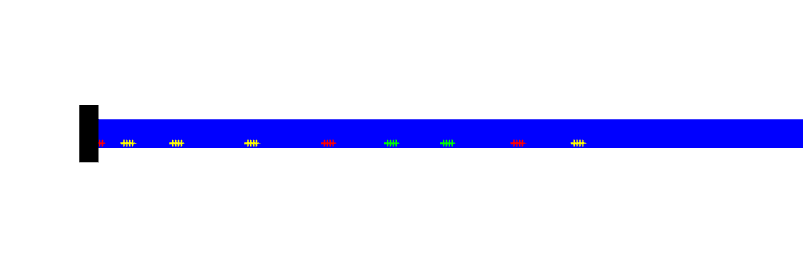
\includegraphics[scale=0.5]{images/SafetyFocussedQueue.png}
  \caption{Screenshot of a simulation run using the SafetyFocussed policy. The lead yellow boat to the right is travelling very slowly causing all the other boats to queue slowly behind it.}
  \label{experiments:safety_queue_screenshot}
\end{center}
\end{figure}

\section{Future Work}
There is no way for this project to exhaust all that the data produced can tell us. There are plenty of other experiments to try and this section gives some suggestions.

The analysis of the data could be made more sophisticated. The Safety experiment suggests that the analysis so far is over-reliant on the use of averages. A further study could look harder at the distribution of crash counts, speeds and locations.

A further study could look at the sensitivity of the data to some of the constants used. For example, crashes cause a delay of 10 ticks. This is a rough guess about the delay a crash causes. It would be very interesting to see how the results changes if crashes were made more punishing and delay boats for longer.

Finally, the launch schedules followed are all follow the same pattern of a fixed delay between boats and the use of a fixed control policy. It would be interesting to examine the launch schedules that match the traffic patterns of the actual Cam much more closely. Another way to improve the safety and efficiency of a cox might be for different types of boats to follow different control policies. So a cox that is aiming to move quickly could follow the Overtaking policy while coxes aiming to move below a certain threshold should follow the more conservative SafetyFocussed policy.

This concludes the look at the data produced by the simulation under different parameters. As the Future Work section shows there still much more that could be studied. Unfortunately time will not allow us to go any further for this report.